\documentclass[conference]{IEEEtran}
% \IEEEoverridecommandlockouts
% The preceding line is only needed to identify funding in the first footnote. If that is unneeded, please comment it out.
\usepackage[utf8]{inputenc} % allow utf-8 input
\usepackage{cite}
\usepackage{amsmath,amssymb,amsfonts}
\usepackage{algorithmic}
\usepackage{graphicx}
\usepackage{textcomp}
\usepackage{xcolor}
\usepackage{hyperref}
%% \usepackage{natbib}

\usepackage{listings}
\lstdefinestyle{lua}{
  language=[5.3]Lua,
  basicstyle=\ttfamily,
  keywordstyle=\color{magenta},
  stringstyle=\color{blue},
  commentstyle=\color{black!50}
}
% solarized
\lstset{
    % How/what to match
    sensitive=false,
    % Extra margin on line (align with paragraph)
    xleftmargin=\parindent,
    % Put extra space under caption
    belowcaptionskip=1\baselineskip,
    % Break long lines into multiple lines?
    breaklines=true,
    % Show a character for spaces?
    showstringspaces=false,
    tabsize=2
}

\definecolor{eclipseStrings}{RGB}{42,0.0,255}
\definecolor{eclipseKeywords}{RGB}{127,0,85}
\colorlet{numb}{magenta!60!black}
\lstdefinelanguage{json}{
    basicstyle=\normalfont\ttfamily,
    commentstyle=\color{eclipseStrings}, % style of comment
    stringstyle=\color{eclipseKeywords}, % style of strings
%    numbers=left,
    numberstyle=\scriptsize,
    stepnumber=1,
    numbersep=8pt,
    showstringspaces=false,
%    breaklines=true,
%    frame=lines,
    string=[s]{"}{"},
    comment=[l]{:\ "},
    morecomment=[l]{:"},
    literate=
        *{0}{{{\color{numb}0}}}{1}
         {1}{{{\color{numb}1}}}{1}
         {2}{{{\color{numb}2}}}{1}
         {3}{{{\color{numb}3}}}{1}
         {4}{{{\color{numb}4}}}{1}
         {5}{{{\color{numb}5}}}{1}
         {6}{{{\color{numb}6}}}{1}
         {7}{{{\color{numb}7}}}{1}
         {8}{{{\color{numb}8}}}{1}
         {9}{{{\color{numb}9}}}{1}
}

\def\BibTeX{{\rm B\kern-.05em{\sc i\kern-.025em b}\kern-.08em
    T\kern-.1667em\lower.7ex\hbox{E}\kern-.125emX}}
\begin{document}

\title{SD-BLS: Privacy Preserving Selective Disclosure and Unlinkable Revocation of Verifiable Credentials\\
%% {\footnotesize \textsuperscript{*}Note: Sub-titles are not captured in Xplore and should not be used}
\thanks{Dyne.org Foundation}
}

\author{\IEEEauthorblockN{1\textsuperscript{st} Denis Roio}
\IEEEauthorblockA{
% \textit{dept. name of organization (of Aff.)} \\
\textit{Dyne.org Foundation}\\
Amsterdam, The Netherlands \\
jaromil@dyne.org}
\and
\IEEEauthorblockN{2\textsuperscript{nd} Rebecca Selvaggini}
\IEEEauthorblockA{
\textit{dept. of Mathematics} \\
\textit{University of Trento}\\
Trento, Italy
}
\and
\IEEEauthorblockN{3\textsuperscript{rd} Andrea D'Intino}
\IEEEauthorblockA{
% \textit{dept. name of organization (of Aff.)} \\
\textit{Forkbomb B.V.}\\
Copenhagen, Denmark \\
info@forkbomb.eu}
}

\maketitle

\begin{abstract}

It is of critical importance to design digital identity systems that
ensure the privacy of citizens as well protect them from issuer
corruption. Unfortunately, what Europe's and USA's public sectors are
currently developing does not offer such basic protections. Aiming at solving this issue, we propose a method for untraceable selective disclosure and privacy preserving revocation of digital credentials, utilizing
the unique homomorphic characteristics of second order Elliptic Curves
and Boneh-Lynn-Shacham (BLS) signatures operated on them. Our approach
ensures that users can selectively reveal only the necessary
credentials, while protecting their privacy across multiple
presentations.  We also aim to protect users from issuer corruption, by making it possible to apply a threshold for revocation to require collective agreement among multiple revocation issuers.

\end{abstract}

\begin{IEEEkeywords}
Privacy, Selective disclosure, BLS signatures, Digital credentials
\end{IEEEkeywords}

\section{Introduction}
Digital identity systems implement credential issuance and presentation mechanisms so that a person (holder) can voluntarily disclose his or her own acquired skills, professed attributes, or completed accomplishments. Credentials are signed by issuer authorities and encapsulated within various forms of digital proofs to be held in digital wallets, empowering individuals to reveal only chosen details to designated recipients, to limit data exposure and permit a user-controlled release of information.

Such systems are known as selective disclosure and this article aims at improving their cryptography to adhere to basic privacy-by-design standards.

\subsection{State of the art}

Selective disclosures are being used by nation states across the world in their next generation identity systems, for instance EIDAS2.0 in Europe where the European Digital Identity Wallet Architecture and Reference Framework\cite{eudi-arf} mandates the use of SD-JWT\cite{sd-jwt} and mDOC \cite{mdoc}. Unfortunately both SD-JWT and mDOC adopt for their cryptography just Hash-Based Message Authentication Codes (HMAC) to generate proofs, and they can be easily traced (non-unlinkability).

In North America the efforts concentrate on the adoption of the the BBS+ algorithm\cite{bbs+} leveraging its Zero Knowledge Proof properties and applied to W3C Verifiable Credentials\cite{w3c-vc} to obtain an higher degree of privacy.

The different choices in data formats in these two approaches is irrelevant in relation with cryptography, being it JSON Web Tokens or W3C Verifiable Credentials and does not impact the privacy level. But the cryptography adopted determines the adequacy to face three important threats that can render an algorithm unsuitable to be used in real world situations.

\subsection{Threats considered}

\paragraph{Linkability}

The EUDI-ARF standard dictates that credentials \textit{issued} to a holder, can be \textit{presented} (in the form of a verifiable presentation) to a relying party in order to have one or more attributes verified. Every verifiable presentation includes one or more HMAC(s), formatted in SD-JWT: the HMACs are identical each time a verifiable presentation is produced from a certain credential. This makes possible for colluding relying parties, or to malicious actors, to trace a holder's identity by collecting, exchanging and confronting verifiable presentations. In order to preserve the privacy of a credential holder the disclosures presented by the wallet should not be traceable across different presentations (unlinkability). This threat appears to be well mitigated by BBS+ through its Zero Knowledge Proof implementation.

\paragraph{Privacy breach of revocation lists}

There is no privacy-preserving revocation system designed, either in EUDI-ARF, or in W3C-VC and BBS+. The approach followed for the revocation is that of the status (revocation) lists \cite{status-lists} for W3C-VC and EUDI-ARF is investigating a similar method. The use of a certificate status lists (CRL) presents issues related primarily to privacy \cite{CRL}, because sensitive information about holders leaks from the list. This is partially mitigated by expiration dates, in cases where credentials can be short-lived (typically less important credentials), but not applicable with digital identification documents such as ID, driving license, passport and social security numbers, which typically have longer or no expiration time. In case the choice of strategy for revocation is left open to developers, the risk for major privacy breaches may occur, for example with the adoption of public status lists \cite{crlcomparison}. Based on these arguments, we believe that anonymous revocations are a \textit{sine qua non}e condition to guarantee a sufficient level of privacy in digital identities and credentials. Our approach is that of designing a privacy-preserving revocation mechanism to remove the leak of holder's information.

%% - https://github.com/ministero-salute/it-dgc-verificaC19-android/issues/103
%% - https://osf.io/preprints/lawarxiv/yc6xu


\paragraph{Revocation issuer corruption}

If the choice of interactive revocation is left to a single issuer, one may unilaterally choose to revoke credentials, without being subject to revision or having to seek consensus with a quorum of issuers. This situation leads to security issues in case Issuers are corrupted and make a weaponized use of digital revocations to persecute engaged individuals. Such a condition becomes a real concern for journalists or activists living under dictatorial regimes that may arbitrarily revoke their credentials, or even ID cards and passports. Similarly, a security breach of an issuer service, would result in similar threats. We mitigate this risk by introducing the possibility for threshold issuance of revocation keys.

\section{Overview}

\subsection{Key contributions}
The  cryptographic scheme described in the paper, name \textit{SD-BLS} for brevity,  takes inspiration by modern zero knowledge proofs schemes  such as \cite{bbs+}BBS signatures or Coconut\cite{coconut}.  The paper aims to employ some of the properties of the said schemes, overcome some of the shortcomings of  SD-JWT and mDOC formats, mainly the non-unlinkability of credentials, proposing a novel cryptographic approach to similar data structures. Furthermore SD-BLS proposes novel anonymous cryptographic revocation flow for verifiable credentials, that aims to solve the privacy issues posed by status and revocation lists.

\paragraph{Unlinkabe selective disclosure}
Similarly to the SD-JWT and mDOC formats, SD-BLS produces an array of claims:  the elements of the array are individually signed by the issuer. In SD-BLS the signature(s) replace the HMAC. Using the homomorphic properties of this curve SD-BLS enables the holder to produce a different \textit{presentation} each time they want to prove a claim. A credential presentation in SD-BLS is in fact a zero knowledge proof offering similar cryptographic properties as \cite{bbs+}BBS signatures or Coconut\cite{coconut} proofs. Given the zero knowledge proof properties of the scheme, SD-BLS can be used to verify credentials off and on blockchain.

\paragraph{Anonymous cryptographic revocation}
SD-BLS proposes a novel approach to credential revocation: the data published by the revocation issuer will produce cryptographic material that contains no information about and is  never linkable to the holder. The cryptographic revocation material allows anyone to verify if an SD-BLS proof produced by a credential holder has been revoked by one or multiple issuers. The unlinkability, and thus anonymity of the cryptographic revocation,  allows the revocation issuer to publish revocations off or on blockchain.

\subsection{Applications}
In this section we present some applications and use cases for digital identity and credentials, that could benefit from using the unlinkability and anonymous revocation of the the SD-BLS scheme.

\paragraph{Digital identity}
The focus of the EUDI-ARF specifications is identity documents: it defines mechanisms and data structures to issue a Personal Identification (PID) as well as digital driving licenses. Similarly, the US government is experimenting with W3C-VC and mDOC for cross-states interoperable driving licenses. SD-BLS data format is similar to SD-JWT and mDOC, offering selective disclosure and adding unlinkability and anonymous revocation.

\paragraph{Academic credentials}
Diploma and academic credentials are among the core offerings of EBSI as well as a primary research target of the W3C VC working group.

\paragraph{KYC/AML}
We are unaware of standardization efforts for interoperable credentials in the fields of "Know Your Customer" (KYC) and Anti Money-Laundering (AML) certifications. We are aware of solution providers experimenting with W3C-VC for AML applications.

\paragraph{Generic \textit{light} credentials}
As the digital identity and verifiable credential technologies are maturing, they are being considered for usage in less privacy concerning applications, such subscriptions and membership and fidelity cards.

\paragraph{Verifiable credentials on Blockchain}
Similarly to other zero knowledge proof schemes, SD-BLS can be used on blockchain.
\begin{itemize}
    \item A verifiable presentation can be used by a smart-contract to verify if one or more holder's claim match the requirement needed to process a transaction. The verifiable presentation is anonymous, therefore its storage in the transaction log doesn't pose privacy issues and is GDPR compatible.
    \item Issuers can publish their cryptographic revocation lists on chain, allowing smart-contracts to verify the status of a credential, still granting unlinkability.
    \item The issuer's public keys can also be published on-chain, although this does not represent a novelty.
\end{itemize}

It's worth mentioning that, while the verifiable presentation is itself unlinkable to the holder's blockchain address, the unlinkability of the holder to their blockchain address at verification phase, needs to be addressed within the blockchain protocol used: this issue is out of scope in this paper.

\section{Implementation}

In this section we will provide a detailed description of the algorithm we propose for selective disclosure and unlinkable revocation using BLS signatures.

\subsection{Notations and assumptions}

We will adopt the following notations:
\begin{itemize}

\item $\mathbb{F}_p$ is the prime finite field with $p$ elements
  (i.e. of prime order $p$);

\item $E$ denotes the (additive) group of points of the curve
  BLS381-12 \cite{bls381-12} which can be described with the
  Weierstrass form $y^2=x^3 + 16$;

\item $E_T$ represents instead the group of points of the twisted
  curve of BLS381-12, with embedding degree $k=12$. The order of
  this group is the same of that of $E$;

\end{itemize}

We also require defining the notion of a cryptographic
pairing. That is defined as a function $e:
\mathbb{G}_1\times\mathbb{G}_2\to \mathbb{G}_T$, where
$\mathbb{G}_1,\mathbb{G}_2$ and $\mathbb{G}_T$ are all groups of same
order $n$, such that satisfies the following properties:

\begin{itemize}

\item [i.] \emph{Bilinearity}, i.e. given $P_1,Q_1\in\mathbb{G}_1$
  and $P_2,Q_2\in\mathbb{G}_2$, we have
  \begin{align*}
    e(P_1+Q_1,P_2) = e(P_1,P_2)\cdot e(Q_1,P_2) \\
    e(P_1,P_2+Q_2) = e(P_1,P_2)\cdot e(P_1,Q_2)
  \end{align*}

\item[ii.] \emph{Non-degeneracy}, meaning that for all
  $g_1\in\mathbb{G}_1, g_2\in\mathbb{G}_2$, $e(g_1,g_2)\ne
  1_{\mathbb{G}_T}$, the identity element of the group
  $\mathbb{G}_T$;

\item[iii.] \emph{ Efficiency}, so that the map $e$ is easy to
  compute;

\item[iv. ] $\mathbb{G}_1\ne \mathbb{G}_2$, and moreover, that
  there exist no efficient homomorphism between $\mathbb{G}_1$ and
  $\mathbb{G}_2$.

\end{itemize}

For the purpose of our protocol we will have $\mathbb{G}_1 = E_T$ and
$\mathbb{G}_2 = E$, and $\mathbb{G}_T\subset \mathbb{F}_{p^{12}}$ is
the subgroup containing the $n$-th roots of unity, where $n$ is the
order of the groups $E$ and $E_T$. Instead $e: E_T \times E\to
\mathbb{G}_T$ is the \emph{Miller pairing}, which in our work is
encoded as the method \verb!miller(ECP2 P, ECP Q)!. \\


\subsection{Issuance} \label{issuance}

As for other well known algorithms BLS signing will work following
three main steps:
\begin{itemize}

\item \textbf{Key Generation phase.} For an issuer who wants to sign
  a credential $m$, a secret key $sk$ is a random number chosen
  uniformly in $\mathbb{F}_n$, where $n$ is the order of the
  groups $\mathbb{G}_1, \mathbb{G}_2, \mathbb{G}_T$. The
  corresponding public key $pk$ is the element $sk\cdot G_2\in
  E_T$;

\item \textbf{Signing phase.} The credential $m$ is first hashed into
  the point $U\in E$, which in our scheme is done by the method
  \verb!hashtopoint!; the related signature is then given by $\sigma =
  sk\cdot U$;

\item \textbf{Verification phase.} For an other user that wants to
  verify the authenticity and the integrity of the message $m$, it
  needs to

  \begin{itemize}

  \item [1.] parse $m, pk$ and $\sigma$

  \item [2.] hash the message $m$ into the point $U$ and then
    check if the following identity holds,

    \[
    e(pk,U) = e(G_2,\sigma)
    \]

  \end{itemize}
If verification passes it means that $\sigma$ is a valid signature for
$m$.
\item \textbf{Proof of correctness} By using the definitions of the elements involved and exploiting the property of the pairing $e$ we have
\[
\begin{split}
    e(pk,U) &= e(sk\cdot G_2, U) \\
            &= e(G_2,U)^{sk}\\
            &= e(G_2,sk\cdot U)\\
            &= e(G_2,\sigma)
\end{split}
\]

\end{itemize}

BLS signatures also support aggregation: it is possible to aggregate a collection of multiple signatures $\sigma_i$ (each one related to a different message $m_i$) into a singular new object $\sigma$, that can be validated using the respective public keys $pk_i$ in a suitable way.

Since $\sigma_i\in G_1 \forall i$, the algorithm has an homomorphic property. We exploit this property to add a revocation signature into the signed credential.

We create a new secret key $rev$ with public key $r_2$, then compute the point $r_1 \in \mathbb{G}_1$ and signature of the claim $\sigma_{rev}$ to add to the issuer signature:
\begin{equation*}\label{rev_agg}
    \begin{split}
        r_2 &= rev \cdot G_2 \\
        r_1 &= rev \cdot G_1 \\
        \sigma_{rev} &= rev \cdot U\\
        \sigma &= sk\cdot U + \sigma_{rev}\\
   \end{split}
\end{equation*}
The set of all the signed claims will be:
\begin{equation*}
   \mathcal{C} = \big\{ \{ r_{1i}, r_{2i}, \sigma_i \} : i\in claims  \big\}
\end{equation*}

At the end of this phase the holder is sent the \textit{signed claims}
to be stored in a private wallet, while the issuer stores
a list of \textit{revocations}, associated with an identifier of the holder and the specific credential, into a private database that can be used later to
issue revocations.



\subsection{Presentation} \label{presentation}

As we have done in the issuance phase (\ref{issuance}), we exploit the
homomorphic property of BLS signatures once again, but this time to
render the presented signature unlinkable (impossible to trace across
multiple presentations) by adding a "blinding factor" signature to the
one provided by the issuer.

Let $\mathcal{H}$ denote a cryptographic hash function (e.g. SHA-256) and let $\varepsilon$ be an integer chosen uniformly at random that serves as the blinding factor.
Using the same technique of the Tripartite Diffie-Hellman Key Exchange \cite{tripartite} we construct a secret that is binded to the blinding factor, the Issuer public key and the "revocation point" $r_1 = rev \cdot G_1$ computed in the issuance phase:

\begin{equation}\label{tau_f}
    \tau = \mathcal{H}(e(A.pk, r_1)^{\varepsilon})
\end{equation}

When the holder needs to disclose a particular claim $m$ we construct the credential proof as follow:
let $\sigma$ be the signature of the claim provided by the Issuer, then apply the blinding factor to the signature using the secret $\tau$
\begin{equation}\label{claim.s}
    s = \sigma + sign(\tau, m)
\end{equation}
and the corresponding public key computed as
\begin{equation*}
    p = r_2 + G_2 \cdot \tau
\end{equation*}
where $r_2$ is the revocation key linked to the claim.
We also attach the public key $r = G_1 \cdot \varepsilon$ that correspond to the secret key $\varepsilon$.

\subsection{Verification}

Credential verification is made by checking that the issuer has signed the blinded proof being presented. In order to do that the credential issuer's public key must be added to the proof.\\
As explained in section \ref{presentation} we can consider the credential proof as a collection of tables of the following form:
\begin{equation*}
    c_p = \{id, p, r, s \}
\end{equation*}
where $s$ and $p$ are respectively the signature and the public key of the credential proof of the string $id$
after verifying the status of the revocation, we can check the validity of the presented claim computing the key
\begin{equation*}
    pk = A.pk + p
\end{equation*}
and verify the bls signature.

\subsubsection{Proof of correctness}
% (questa è praticamente una proof dell'homomorphic property...)
The signature $s$ is given by
\begin{equation*}
\begin{split}
    s &= \sigma + sign(\tau, id) \quad \text{where} \\
    \sigma &= sign(A.sk, id) + sign(rev, id) \\
    \text{so} \quad s &= A.sk U + rev U + \tau U
\end{split}
\end{equation*}
where $U$ is the mapping of the string $id$ in the group $G_1$.\\
Recalling the verification formula, it holds that:
\begin{equation*}
\begin{split}
 e(pk, U) &= e(A.skG_2 + revG_2 + \tau G_2, U) \\
 &= e(A.skG_2 + revG_2)\cdot e(\tau G_2, U) \\
 &= e(A.skG_2, U) \cdot e(revG_2, U) \cdot e(\tau G_2, U) \\
 &= e(G_2, A.sk U) \cdot e(G_2, rev U) \cdot e(G_2, \tau U) \\
 &= e(G_2, A.sk U) \cdot e(G_2, rev U + \tau U) \\
 &= e(G_2, A.sk U + rev U + \tau U) \\
 &= e(G_2, s) \\
\end{split}
\end{equation*}
where each equality holds for the bilinearity of the Miller loop.

\subsection{Revocation}

To make sure no revocation has been emitted for each credential, we update the revocation list from the issuer. A revocation list can be publicly distributed since revocation keys do not provide any information on the identity of holders, unless they are presented in a verification.

Given an element $c_p = \{id, p, r, s \}$ of the credential proof table and the Issuer public key $A.pk$, if the claim id is present in the revocation list we can take the corresponding revocation private key $rev$ and compute the factor $\tau$ as
\begin{equation}\label{tau}
        \tau = \mathcal{H}(e(A.pk, r)^{rev})
\end{equation}

The equation \eqref{tau} gives the same result as \eqref{tau_f} since using the bilinearity of the pairing \cite{tripartite} we have:
\begin{equation*}
    \begin{split}
        \tau &= \mathcal{H}(e(A.pk, r)^{rev}) \\
        &= \mathcal{H}(e(A.pk, G_1 \cdot \varepsilon)^{rev}) \\
        &= \mathcal{H}(e(A.pk, G_1)^{rev \cdot \varepsilon}) \\
        &= \mathcal{H}(e(A.pk, G_1 \cdot rev)^{\varepsilon}) \\
        &= \mathcal{H}(e(A.pk, r_1)^{\varepsilon})
    \end{split}
\end{equation*}

Then we can verify if a credential claim has been revoked checking first if the revocation public key match:
\begin{equation*}
    G_2 \cdot rev = p - G_2 \cdot \tau
\end{equation*}
and then verify the following signature with the issuer's public key (pk):
\begin{equation}\label{sig_minus}
    sig = s - sign(\tau, id) - sign(rev, id)
\end{equation}
This signature should be verified with the issuer's pk since:
\begin{equation*}
    \begin{split}
        s &= \sigma + sign(\tau, id) \quad \text{from \eqref{claim.s}} \\
        &=  sign(sk, id) + sign(rev, id) + sign(\tau, id)
    \end{split}
\end{equation*}
then exploiting the homomorphic property of BLS signature
we got that $sig$ in \eqref{sig_minus} is signed using the issuer's private key.

\subsection{Threshold Revocation}

In order to split responsibilities over interactive revocation we introduce an optional threshold over the revocation key, plus we split the functionality of \textit{credential issuance} from that of \textit{revocation issuance}, now operated by different peers.

This is implemented via an interactive process facilitated by a third party trustee who should be:
\begin{itemize}
    \item never entitled to publish revocations
    \item connected to credential issuers to complete any credential signature
    \item never informed about the identity of credential holders
    \item regularly connected to revocation issuers to distribute shares
\end{itemize}

Such a trustee will be in contact with \textit{credential issuers} for the signature of credentials: it will create the $rev$ revocation key while concealing it from them. The trustee then proceeds creating the $\sigma_{rev} = rev \cdot U$ revocation signature and the $r_1 = rev \cdot G_1$ projection as detailed in the issuance phase \eqref{rev_agg}. Finally the revocation trustee will distribute $\sigma_{rev}$ and $r_1$ to issuers for further processing into the final signed credential.

The trustee will then proceed asynchronously to split the revocation key into shares using a public verifiable secret sharing (PVSS \cite{pvss_schoenmakers}) implementation and distribute these shares to all revocation issuers. In order to issue a revocation, a configurable quorum of peers among the revocation issuers will need to reconstruct the secret revocation key and publish it.

\section{Benchmarks}

We implemented the flows for credential issuance, presentation, verification and revocation for lab tests using Zenroom \footnote{Zenroom home: https://zenroom.org}, a secure isolated execution environment implementing advanced cryptography transformations. The reference implementation for this paper is published on a public repository \footnote{SD-BLS github repository: https://github.com/dyne/sd-bls}. All benchmarks were executed on a 6th gen. Intel PC running tests on a single i7 3.40GHz core and making no use of hardware acceleration.

Lab measurements on a growing number of claims show that issuance is less computation heavy and that the production of proofs and their verification need approximately the same resources, as shown in figure \ref{fig:issueproveverify}.

\begin{figure}
    \centering
    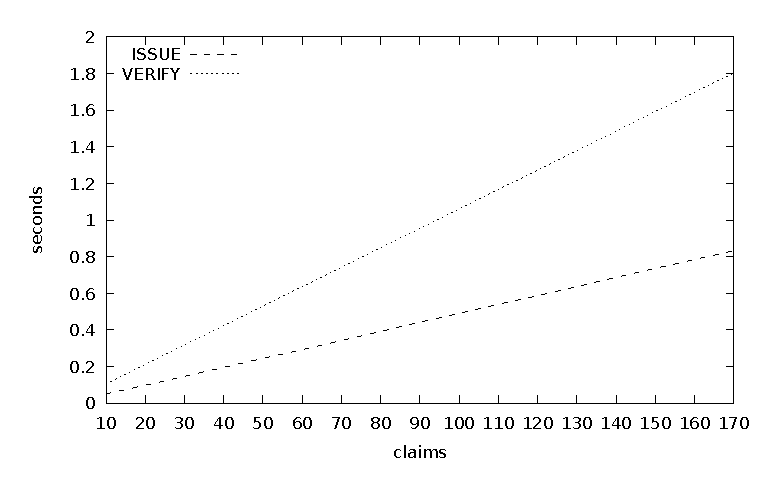
\includegraphics[width=1\linewidth]{issueproveverify.eps}

    \caption{Speed comparison of issue, prove and verify}
    \label{fig:issueproveverify}
\end{figure}

Based on our benchmarks, the resulting data objects sizes are:
\begin{itemize}
    \item Claim: 322 Bytes
    \item Proof:  226 Bytes
    \item Revocation: 64 Bytes
\end{itemize}

The computational cost grows for the verification phase with the presence of a cryptographic revocations list. We assume that revocations are grouped by claim type or credential structure, for instance all revocations of a certain claim (e.g.: "is above 18" or "is a Danish citizen") for any holder are published in the same list: this will not degrade the level of privacy and will group all the revocations in smaller lists.

Lab measurements of the time taken by a single proof verification process to operate on a growing number of revocations demonstrate that there is a linear growth, as shown in figure \ref{fig:verifyrevocations}.

\begin{figure}
    \centering
    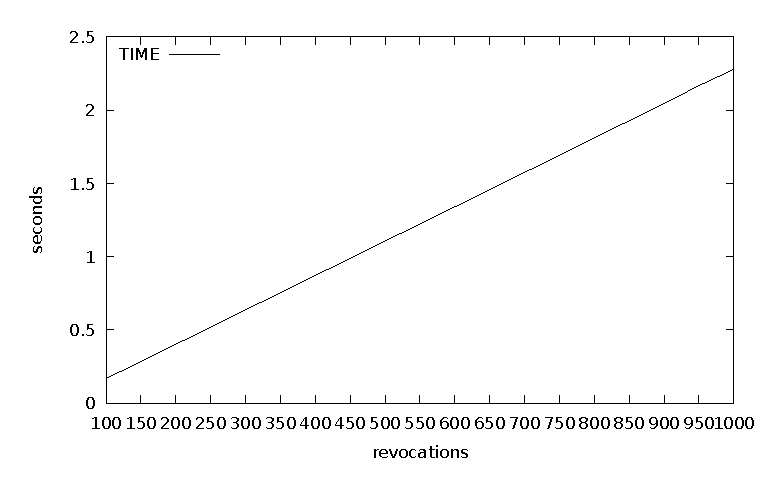
\includegraphics[width=1\linewidth]{verifyrevocations.eps}

    \caption{Speed of verification of a claim over multiple revocations}
    \label{fig:verifyrevocations}
\end{figure}

At last we measure the binary hamming distance between unlinkable proofs of the same credential signed by the same issuer. We performed this test without using any special random generator.  This measurement should serve as a quick evaluation of the "randomness" of all blinded contents constituting a proof: the signature, the issuer's public key and the revocation's public key, from this benchmark the claim's identifier is excluded. The results are shown in figure \ref{fig:hamming} and include an overlay of frequency values taken from the comparison of two random values. This benchmarks show that the binary hamming distance between different proofs is the same as the one between two random values of the same length generated by the same PRNG.

\begin{figure}
    \centering
    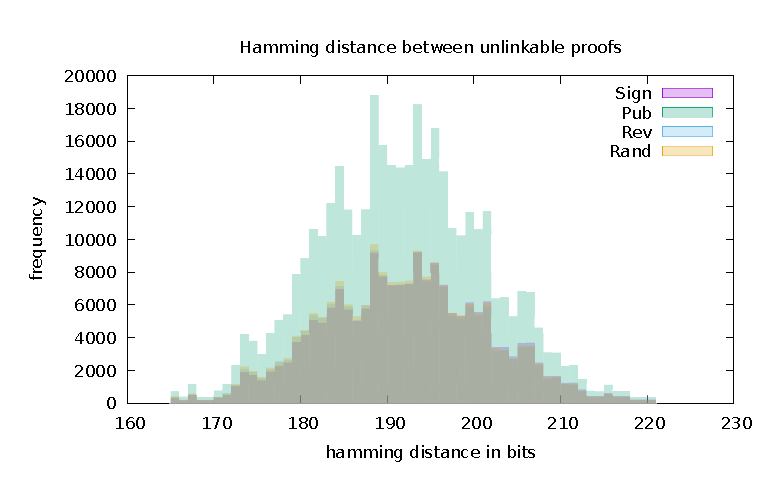
\includegraphics[width=1\linewidth]{hamming.eps}

    \caption{Frequency of hamming distance between unlinkable proofs}
    \label{fig:hamming}
\end{figure}

%---------

\section{Conclusion}
\subsection{Security considerations}

The revocations database is privacy and corruption sensitive (by our previous definition of issuer corruption) and it should be securely stored by each Issuer. This is mitigated by the optional adoption of threshold revocation. When using threshold revocation there is still the need for a \textit{revocation trustee} who may be a single point of failure if allowed to publish revocation keys dishonestly collected during the process of credential issuance.

BLS signatures and the proof system obtained with credentials are
considered secure by assuming the existence of random oracles
\cite{random-oracle}, together with the decisional Diffie-Hellman
Problem (DDH) \cite{DDH-problem}, the external Diffie-Hellman Problem
(XDH), and with the Lysyanskaya-Rivest-Sahai-Wol Problem (LRSW)
\cite{lrsw-assumption}, which are connected to the Discrete
Logarithm. In fact, under these assumptions, we have that our protocol
satisfies unforgeability, blindness, and unlinkability.

The SD-BLS implementation we are presenting in this paper is
demonstrated using the BLS381-12 curve \cite{bls381-12} also adopted
by ETH2.0. Debating the choice of BLS381-12 is beyond the scope of
this paper, but is worth mentioning that we can easily switch using the BLS461 curve based on a 461 bit prime, hence upgrading our
implementation to 128 bit security \cite{updating-key-pairings}
against attacks looking for discrete logs on elliptic curves
\cite{discrete-log-attack}.

The future growth
of quantum-computing technologies may be able to overcome the Discrete
Logarithmic assumptions by qualitatively different computational
means and SD-BLS may then be vulnerable to quantum-computing attacks. However this is speculative reasoning on what we can expect from the
future.

\subsection{Future development}
In this section we describe possibilities for expanding the algorithm to cover further applications, which appear promising while requiring further investigation.

\paragraph{Key-value claims}
The focus of the initial version of the SD-BLS algorithm is on claims consisting of fixed and predetermined values (e.g.: "is above 18" or "has M.Sc. in applied cryptography"), whereby a credential could contain multiple claims. This initial version doesn't include the possibility to process claims containing a predetermined part (the \textit{key}) and a variable one (the \textit{value}). We're expecting to be able support \textit{key-value} based claims in the next version of the paper.

\paragraph{Compatibility with EUDI-ARF}
EUDI-ARF dictates that the holder's secret key generation and signatures must occur inside a trusted platform module (TPM). For mobile devices, this limits the secret keys and signatures to those offered, via proprietary APIs by the mobile OS, namely RSA (multiple flavours) and ECDSA on the secp256r1 curve. Currently the TPMs APIs supported by Android and iOS do not support BLS 12381 key generation or signature.
Client-side signatures in EUDI-ARF are mostly used in the authentication process, specifically in the proof of possession required by the OpenID4VCI\cite{OID4VCI} issuance flow, but not in the verification.
Therefore, we can investigate the possibility to use SD-BLS to implement a partially retro-compatible superset of EUDI-ARF, by maintaining the current issuance and verification protocols and using an extended SD-JWT format. Also, because of the unlinkable feature of credentials and revocations in SD-BLS, we can explore useful integrations with the European Blockchain Services Infrastructure (EBSI \cite{ebsi}).


\paragraph{Digital Product Passport}
Efforts in standardization of Digital Product Passport (DPP) are ongoing in both the EU (Cirpass, BatteryPass, Trace4EU) and US (DSCSA). An obstacle to adoption of DPP technologies is the reluctancy of manufacturers to share information about their supply-chain, knowing that the information would become publicly available and immutable due to blockchain storage. While requiring further analysis and investigation, a further development of the SD-BLS scheme could allow creating DPPs built on the zero knowledge proof and selective disclosure principles, which may facilitate the adoption of the technology in the industry.

\paragraph{DAO Technologies}
The SD-BLS math is fully compatible with ETH2.0 and can be computed inside an Ethereum VM. If implemented in solidity, it can be a useful building block for more advanced Distributed Autonomous Organizations (DAO \cite{dao}) that want to authenticate peers using on a set of universally recognizable credentials instead of a key based proof of possession.

% Our preliminary benchmarks suggest that while the computationally heaviest part of cryptographic scheme is the verification, the issuance and the creations of a presentation are computationally relatively inexpensive.

\bibliographystyle{IEEEtran}
\bibliography{references}

\end{document}
